\documentclass[crop,tikz]{standalone}
\usetikzlibrary{backgrounds}
\colorlet{blue}{cyan}
\tikzset{
  inverted/.style = {
    color=white,
    background rectangle/.style={fill},
    show background rectangle
  }
}

\usepackage[european]{circuitikz}
\usepackage{siunitx}

\begin{document}
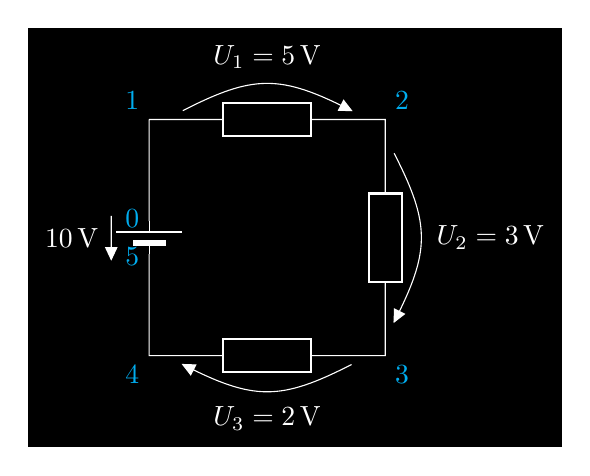
\begin{tikzpicture}[inverted,inverted]
  \draw (0,1.5)
    to[battery2,v_={$\SI{10}{\V}$}] ++(0,-3) node[below left,blue] {4}
    to[R,v<={$U_3=\SI{2}{\V}$}] ++(3,0) node[below right,blue] {3}
    to[R,v<={$U_2=\SI{3}{\V}$}] ++(0,3) node[above right,blue] {2}
    to[R,v<={$U_1=\SI{5}{\V}$}] ++(-3,0) node[above left,blue] {1};
  \node[above left,blue] at (0,0) {0};
  \node[below left,blue] at (0,0) {5};
\end{tikzpicture}
\end{document}
